\documentclass[../../main]{subfiles}

\renewcommand\thesection{\arabic{section}}


\begin{document}

\section{Light Monitoring System} \label{sec:}

There's two ways to detect \emph{light intensity} inside the incubator. One is
to use an array of LDR\footnote{Light Dependent Resistors.} or to use \emph{Esp
Cam} module to capture a picture and process the image to \emph{estimate} the light
intensity. The former makes the hardware part a bit complicated and the latter
method requires to \emph{post process} the image to estimate the light
intensity. But latter method is preferable, because the \emph{Cam} can be used for
other things, such as estimating the \emph{growth} of the seedling\footnote{Even
though, it requires to train a model using TinyML, and would be hard to complete
the implementation, given the time constrain.}.

So, currently we are simply using an array of LDR sensors to gather the light
information through the \emph{multiplexer circuit} we designed in the chapter \ref{chp:auxiliarySystem}.
Figure \ref{fig:ldrSensorImage} depicts the sensor.

\begin{center}
    {\begin{minipage} [c] {0.55\textwidth}

        Specification:

        \begin{itemize}
            \item \textbf{Operating voltage:} $3.3\si{V}$ to $5\si{V}$.
            \item \textbf{Maximum power dissipation:} $600 \si{mW}$.
            \item \textbf{Peak wavelength:} $600 \si{nm}$.
            \item \textbf{Dark resistance:} $0.25 \si{M \ohm}$.
            \item \textbf{Light resistance:} $0.7 \si{k \ohm}$.
        \end{itemize}

    \end{minipage}
    \hfill
    \begin{minipage} [c] {0.35\textwidth}
        \centering
        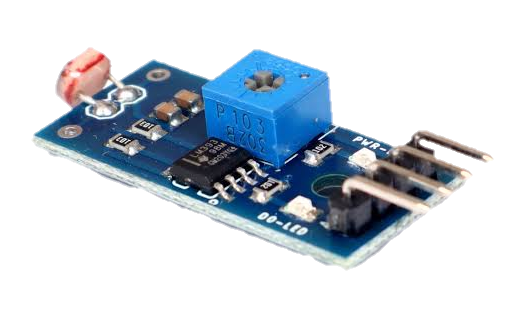
\includegraphics [
            max width = \IGXMaxWidth,
            max height = \IGXMaxHeight,
            \IGXDefaultOptionalArgs,
        ] {pics/ldr_sensor.png}
        \captionof{figure} {
            LDR Sensor.
            \label{fig:ldrSensorImage}
        }
    \end{minipage}\hfill}
\end{center}

\alertNote{
    We are simply using the analog pins of the sensor, even when it it has comparator and
    there's a total of $3$ LDR sensors.
}

\begin{figure}
    \centering
    \includegraphics [
        max width = \IGXMaxWidth,
        max height = \IGXMaxHeight,
        \IGXDefaultOptionalArgs,
    ] {tikzpics/endAbsLightSensingSystem.pdf}
    \captionof{figure} {LDR interfacing using $32$ bit multiplexer.}
    \label{fig:absLightSensingSystem}
\end{figure}

\alertWarning{
    The \emph{BUF} and \emph{0/1} blocks of figure \ref{fig:absLightSensingSystem} are part of
    the \emph{auxiliary system} that is not implemented\footnote{there will be a circuit that
    helps to enable and disable different systems.} yet. Right now the power pins of the sensors
    are tied directly to $3.3\si{V}$.
}

\alertNote{
    \texttt{AO} pins of \emph{LDR} sensors are connected to the \texttt{C0}, \texttt{C1}
    and \texttt{C2} pins of $32$ bit multiplexer.
}

\end{document}
